\documentclass{sigchi}

% Use this command to override the default ACM copyright statement (e.g. for preprints). 
% Consult the conference website for the camera-ready copyright statement.


%% EXAMPLE BEGIN -- HOW TO OVERRIDE THE DEFAULT COPYRIGHT STRIP -- (July 22, 2013 - Paul Baumann)
% \toappear{Permission to make digital or hard copies of all or part of this work for personal or classroom use is 	granted without fee provided that copies are not made or distributed for profit or commercial advantage and that copies bear this notice and the full citation on the first page. Copyrights for components of this work owned by others than ACM must be honored. Abstracting with credit is permitted. To copy otherwise, or republish, to post on servers or to redistribute to lists, requires prior specific permission and/or a fee. Request permissions from permissions@acm.org. \\
% {\emph{CHI'14}}, April 26--May 1, 2014, Toronto, Canada. \\
% Copyright \copyright~2014 ACM ISBN/14/04...\$15.00. \\
% DOI string from ACM form confirmation}
%% EXAMPLE END -- HOW TO OVERRIDE THE DEFAULT COPYRIGHT STRIP -- (July 22, 2013 - Paul Baumann)


% Arabic page numbers for submission. 
% Remove this line to eliminate page numbers for the camera ready copy
\pagenumbering{arabic}


% Load basic packages
\usepackage{balance}  % to better equalize the last page
\usepackage{graphics} % for EPS, load graphicx instead
\usepackage{times}    % comment if you want LaTeX's default font
\usepackage{url}      % llt: nicely formatted URLs
\usepackage[usenames,dvipsnames]{xcolor}
\usepackage[utf8]{inputenc}
\usepackage{tabularx}

% llt: Define a global style for URLs, rather that the default one
\makeatletter
\def\url@leostyle{%
  \@ifundefined{selectfont}{\def\UrlFont{\sf}}{\def\UrlFont{\small\bf\ttfamily}}}
\makeatother
\urlstyle{leo}

\usepackage{etoolbox}
\makeatletter
\patchcmd{\maketitle}{\@copyrightspace}{}{}{}


% To make various LaTeX processors do the right thing with page size.
\def\pprw{8.5in}
\def\pprh{11in}
\special{papersize=\pprw,\pprh}
\setlength{\paperwidth}{\pprw}
\setlength{\paperheight}{\pprh}
\setlength{\pdfpagewidth}{\pprw}
\setlength{\pdfpageheight}{\pprh}

\newcommand{\papertitle}{Password Blur - A Usable and Secure Password Input Method for Mobile Devices}

% Make sure hyperref comes last of your loaded packages, 
% to give it a fighting chance of not being over-written, 
% since its job is to redefine many LaTeX commands.
\usepackage[pdftex]{hyperref}
\hypersetup{
pdftitle={\papertitle},
pdfauthor={LaTeX},
pdfkeywords={password, filter, distortion, shoulder surfing, security},
bookmarksnumbered,
pdfstartview={FitH},
colorlinks,
citecolor=black,
filecolor=black,
linkcolor=black,
urlcolor=black,
breaklinks=true,
}

% create a shortcut to typeset table headings
\newcommand\tabhead[1]{\small\textbf{#1}}

\newcommand{\missing}[1]{\textcolor{Red}{\textbf{(To Do: }\textit{#1})}}

% End of preamble. Here it comes the document.
\begin{document}

\title{\papertitle}

\numberofauthors{1}
\author{
  \alignauthor Zhe Li, Leonhard Mertl, Alice Nguyen, Mario Schneller\\
    \affaddr{Ludwig-Maximilians-Universität München}\\
    \email{\{li.zhe,l.mertl,alice.nguyen,mario.schneller\}@campus.lmu.de}\\
}

% \numberofauthors{4}
% \author{
%   \alignauthor Zhe Li\\
%     \affaddr{Ludwig-Maximilians-Universität München}\\
%     \email{li.zhe@campus.lmu.de}\\
%   \alignauthor Leonhard Mertl\\
%     \affaddr{Ludwig-Maximilians-Universität München}\\
%     \email{l.mertl@campus.lmu.de}\\ 
%   \alignauthor Alice Nguyen\\
%     \affaddr{Ludwig-Maximilians-Universität München}\\
%     \email{alice.nguyen@campus.lmu.de}\\
%   \alignauthor Mario Schneller\\
%     \affaddr{Ludwig-Maximilians-Universität München}\\
%     \email{mario.schneller@campus.lmu.de}\\
% }


 \teaser{
 \centering
     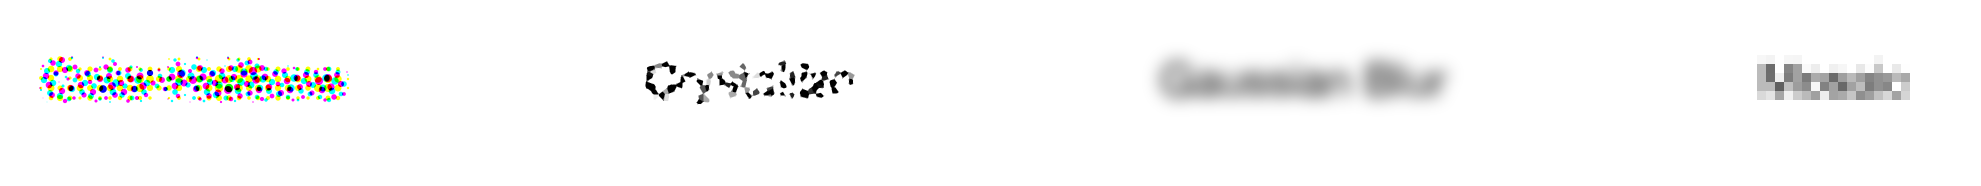
\includegraphics[width=\textwidth]{figures/teaser.png}
     \caption{We explored different filter types to improve the usability and security of the common asterisk-based authentication method on mobile devices (from left to right: Color-Halftone, Crystallize, Gaussian Blur and Mosaic)}
     \label{fig:teaser}
 }


\maketitle

\begin{abstract}

Humans have the ability to understand degraded versions of images, provided they know about the original version of the image. The main focus of this project is to study how this concept can be applied on textual passwords.
As a first step we investigated the topic generally by asking 163 people via an online survey whether they would recognize text elements that have been visually degraded by the Gaussian Blur, Color Halftone, Crystallize and Mosaic filters. As a second step we brought this concept to the context of password input. By conducting an in-depth user study with 25 participants we collected significant quantitative and qualitative feedback. The study contained two practical tasks that investigated the usability and security of the new authentication method and compared it to. traditional alternatives, which are Android/iOS default password entry methods and plain text. The hands-on tasks were followed by a qualitative interview. 
We found, that our filter-based authentication approach is a distinctly more secure alternative to traditional password input methods with its usability performing at a comparably high level. To achieve optimum results we recommend to apply this novel input technique by using the Crystallize filter which showed most promising results in terms of usability and security.
As a next step we propose a long-term field-study to get more detailed insights on human perception of different filter gradations and evaluating this method in an extended scope. 

\end{abstract}

\keywords{Password; Filter; Distortion; Shoulder Surfing; Security; Authentication}

%\category{H.5.2.}{Information Interfaces and Presentation}{User Interfaces -- Input Devices and Strategies
%}


\section{Introduction}
There are more than 2.8 billion internet users world wide \cite{meeker2015internet} which use on average 25 different accounts with 8 log-ins online per day \cite{florencio2007large}. But even with new authentication technologies like finger print sensors or iris scanners, passwords are still the major approach for data protection and privacy in the web \cite{florencio2007large}.
Although passwords are not getting obsolete in the near future, they are far from being perfectly secure. 

Due to the error sensitivity of user inputs on smartphones, the typed characters of a password are shown for a few milliseconds before turning into asterisks. As a consequence basically everybody's private data is at risk to be obtained via shoulder surfing attacks \cite{eiband2017understanding}. Shoulder surfing is by definition "the practice of spying on the user of a cash-dispensing machine or other electronic devices in order to obtain their personal identification number, password, etc." \cite{oxforddicshouldersurfing}.
Besides the security related issues, there are also usability barriers related to traditional authentication methods. Using asterisks to hide passwords from third-parties has the consequence  that users are not able to detect spelling mistakes and therefore have to delete the whole input when they find themselves confronted with incorrect entries.

To challenge this state of the art password input and enhance usability and security for authentication on mobile devices we propose a novel method using image filters to distort the textual password. We investigate if users are able to detect spelling mistakes in their distorted password input and if the distorted passwords can resist shoulder surfing attacks by third-parties. Additionally we evaluate the trade-off between usability and security when applying this method.



\section{Related Work}
The idea using the distortion filters on textual password input to exploit the human sense of cognition is based on previous research. It was found that humans are able to pick a known image out of a larger set, even if they only see a degraded version of the original \cite{burton1999face,gregory1997knowledge,kinjo2000does}.
Harada et al. \cite{harada2006user} and Hayashi et al. \cite{hayashi2008use} used this as a basis to develop graphical user authentication (GUA) mechanisms. Hayashi et al.'s approach is called Use Your Illusion. Images for the GUA are distorted by an Oil Paint filter, which eliminates most details in the images, but preserves some details like colours and rough shapes. The user has to select his chosen image portfolio out of other distorted images to authenticate. As a result, the usability of graphical password schemes is maintained and become resilient to guessing attacks. However, the authors point out that the selection of the best filter for this mechanism requires further investigations.
Von Zezschwitz et al. \cite{von2016you} used the same concept of human recognition for browsing photos securely. Three filter types (Oil Paint, Crystallize, Pixelate (Mosaic)) with three filter strength (none, medium, high) were examined and successfully proven to conceal the pictures’ content. 

Using the findings described above, we decided to use the Crystallize and Pixelate filter for our study. The Oil Paint filter showed to be impractical, because when being applied on text, the distorted characters were still too predictable. As a compensation we decided to add Gaussian Blur that also relies on the concept of blur, but in a more extensive way that allows degrading text as needed for our study. To get even broader results we decided to introduce a fourth filter rooted in the family of the pixelate filters \cite{pixelatefilters}. We chose Color Halftone, a filter that divides the image into rectangles and replaces each rectangle with a circle and is therefore a different jet related filter to Crystallize and Pixelate.

\section{Methodology}

\subsection{Quantitative Online Survey}
Our first study in form of an online survey was not designed to provide us with significant data, but rather to give us feedback from many participants in a short amount of time. Our goal was to get a first feeling for the different filters, filter strengths and overall performance of the participants in security and usability related questions. 
First and foremost, based on the previous work from Hayashi et al. \cite{hayashi2008use} using degraded versions of pictures for the authentication process, we wanted to know if there is a difference in the performance of the participants if they know what a degraded word should mean in contrast an for them unknown word. Furthermore the study should clarify whether there are other factors like password length, random character strings, filter types and filter strengths that could have an impact on the perceptibility of distorted text.

\subsubsection{Survey Design}
In the survey we tested four different filters (Color Halftone, Crystallize, Gaussian Blur and Mosaic) with two strengths each (light and strong) and six questions per condition. As we wanted the survey to be doable in about 10 minutes, each participant had to answer 20 random questions out of a pool of 48 in total. 
We differentiated between usability and security related questions. The usability related questions should clarify whether the participants were able to recognize words known to them, what we call Owner Guessability.
In the security related questions we tested the Guessability of (to the user) unknown words and character strings, the so called Third Person Guessability.

\begin{figure}[h]
    \centering
    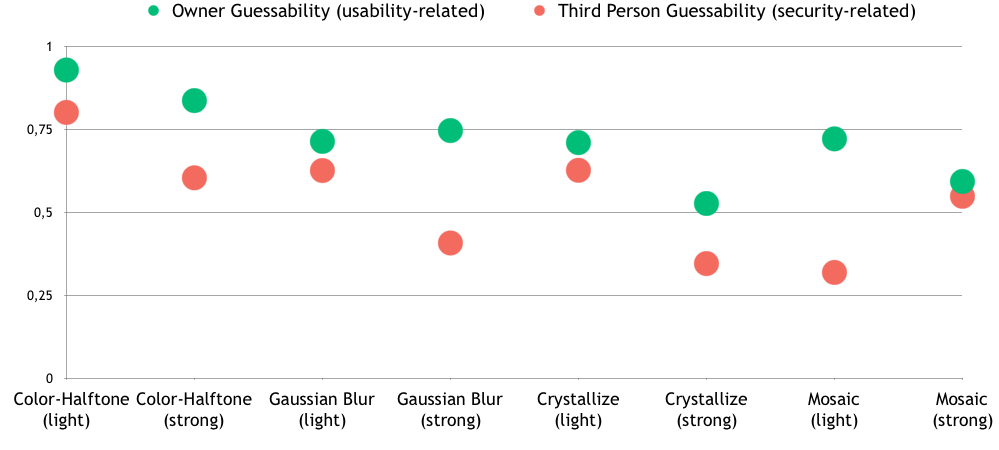
\includegraphics[width=\columnwidth]{figures/figure1.png}
    \caption{Average Levenshtein distance ratio depending on the word length for each condition: Color-Halftone had the highest usability, while Crystallize and Mosaic were the most resistant ones to observations by third persons}
    \label{fig:online-survey_results}
    \vspace{-5mm}
\end{figure}


\subsubsection{Results and Discussion}
In total our survey had 163 participants with each question answered on average more than 67 times. As mentioned before even though there is no significant data, we could see certain trends, which were addressed in a follow-up study.
As seen in figure \ref{fig:online-survey_results}, there seems to be a difference in the Owner Guessability as well as the Third Person Guessability in correlation with both, the filter type and strength. Since we were looking for a filter that has a high usability as well as a high security we chose the filter strengths with the highest Owner Guessability and at the same time lowest Third Person Guessability for our second study.
Moreover the survey data shows clearly that there is a difference when the user knows which word should be shown as the Owner Guessability performed overall better than the Third Person Guessability. We could also see in the data, that there is a big difference in the perceptibility when the word given has an actual meaning rather than random characters.
Based on this first impression a follow-up study was planned, which tested the filters in a real world scenario and aimed for significant data.

\subsection{Quantitative and Qualitative User Study }
With this follow up user study we examined the performance of filter-based password input in terms of usability and security in comparison to traditional plain text and asterisk-based input methods. 

\subsubsection{Study Design}
25 participants, aged between 18 and 32, were recruited via social networks and personal invitation. To allow a more natural setting the participants performed all input related tasks on their own smartphone. Therefore we provided them with a server that had our prototype running and was accessible through the university's wifi.

We used a repeated-measures ANOVA for analysing the data. The study contained 2 practical tasks that collected quantitative data on usability and security and a concluding survey that aimed for qualitative data. 
We used again (1) Color Halftone, (2) Crystallize, (3) Gaussian Blur and (4) Mosaic filters. With the added traditional methods Plain Text and Asterisks we counted 6 conditions in total. For each filter we presented the participant with three different password types: short words, random combinations containing special characters and password phrases. Each of the password types had 2 variants. To eliminate learning effects and to counterbalance the combination of passwords and filters we generated a unique, 36 item long password list for each task and shifted the order of filters for every participant by using a 6$\times$6 Latin square \cite{williams1949experimental}.

Task 1 that investigated the usability, was split into 2 parts. First, the participants had to enter a given password into an input-field and secondly insert the character x at a specific position. For the first part of task 1, the dependent variables were Levenshtein distance (similarity between entry and the actual password) \cite{damerau1964technique, levenshtein1966binary} and entry time. For the second part the dependent variables were editing accuracy (similarity between user entry and the correct position of the x) and editing time. For both parts the independent variables were filter type, password type and entry number.

\begin{figure}[h]
    \centering
    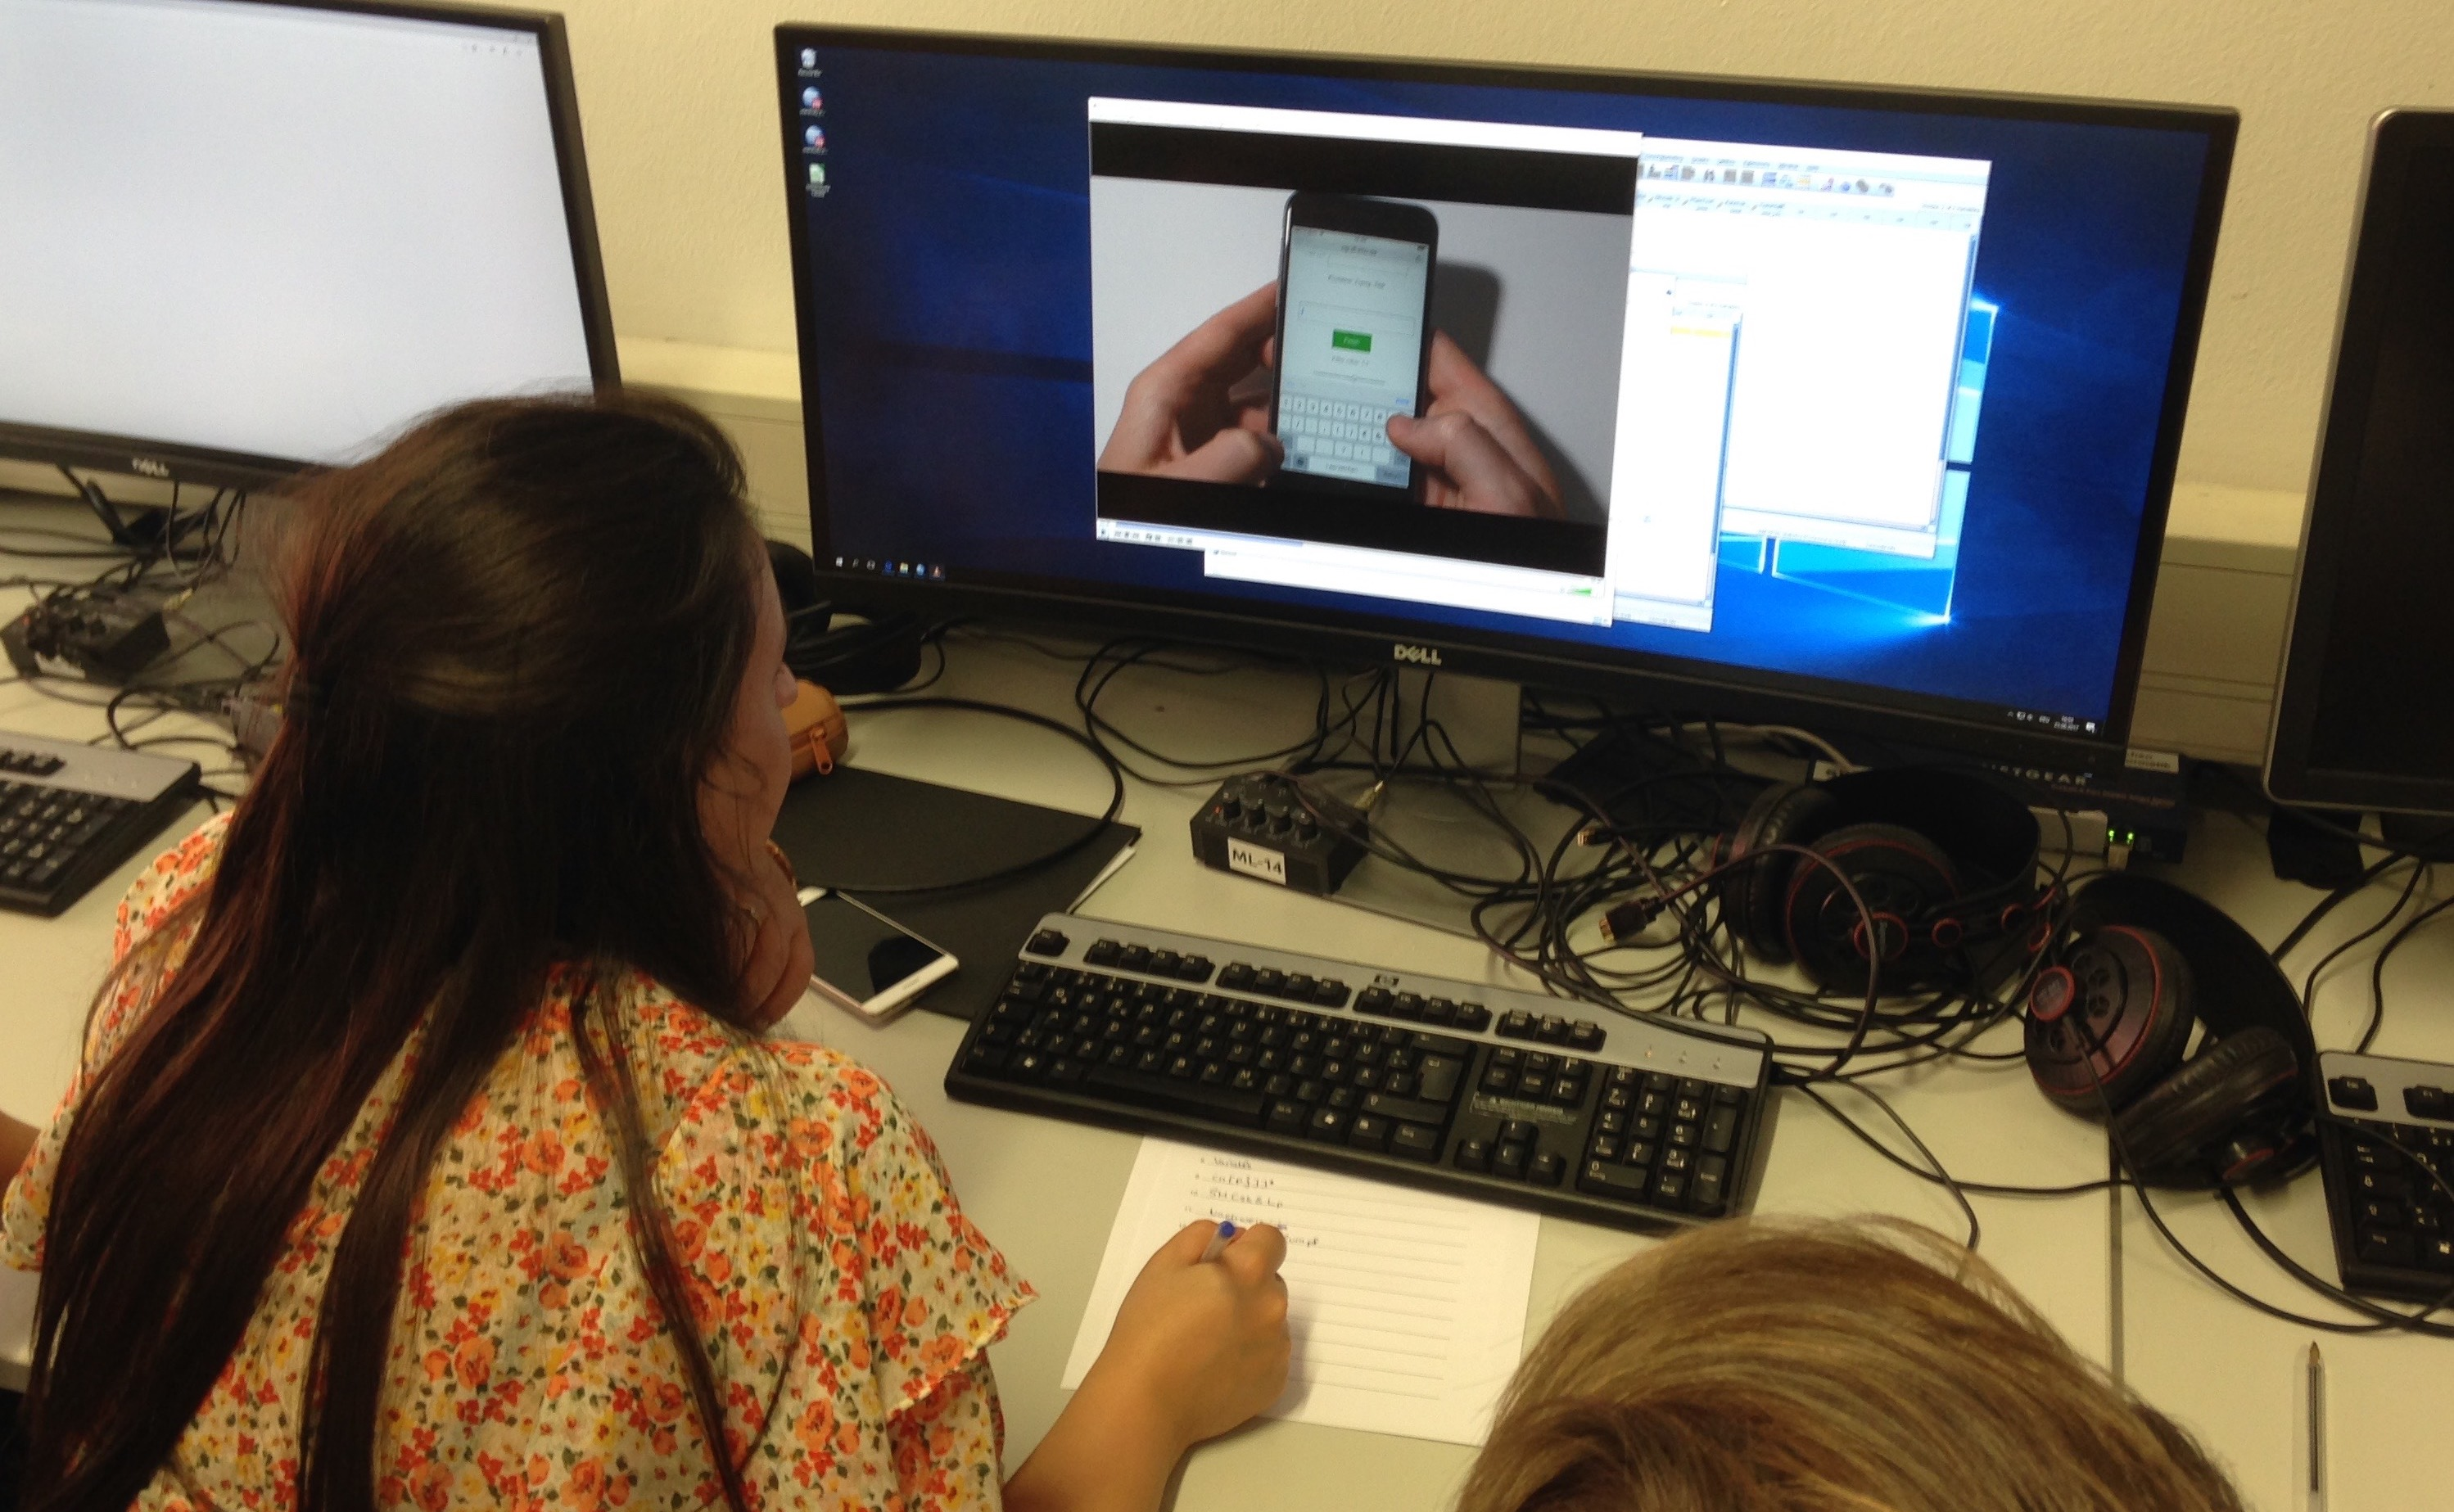
\includegraphics[width=\columnwidth]{figures/studie.jpg}
    \caption{Second part of the study: The participants were asked to look at a recorded video and try to obtain the entered password}
    \label{fig:study}
    \vspace{-1mm}
\end{figure}

Task 2 of the study was considering the security of the different filters and traditional password input methods in the context of shoulder surfing. The participants were asked to act as a shoulder surfer and try to obtain passwords by looking at a recorded video, where a password input procedure was shown in close-up (see figure \ref{fig:study}). The participants noted the observed password with pen and paper and transcribed it to a digital form at a later stage to avoid transcription mistakes. In sum the participants were trying to exploit the password inputs of 36 video clips (see \ref{fig:filters_study_part2}). The dependent variable was the Levenshtein distance (similarity between noted password and the actual password). The independent variables were filter type, password type and entry number.

\begin{figure}[h]
    \centering
    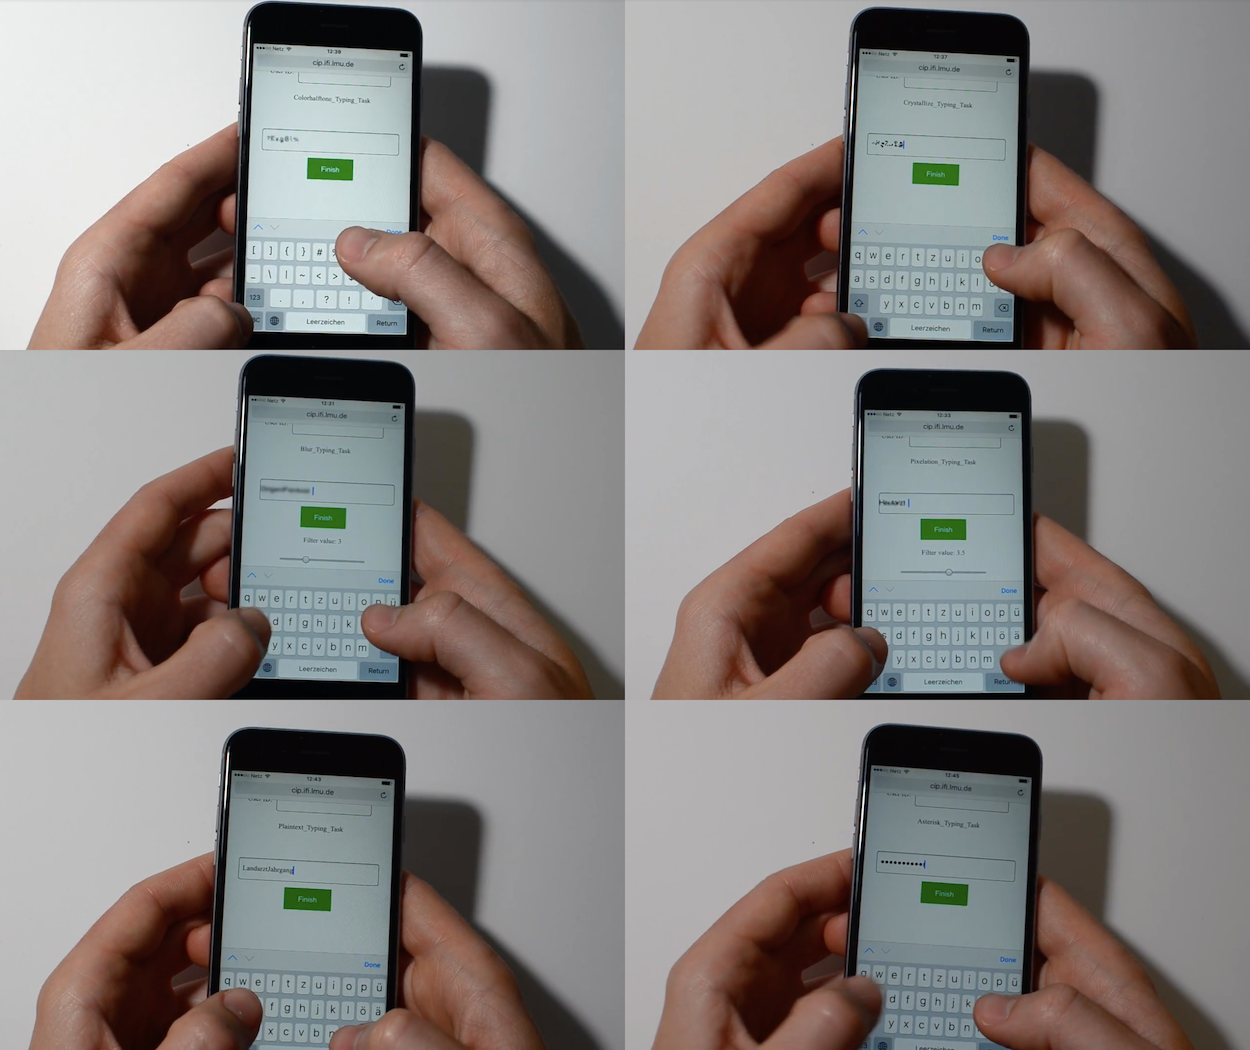
\includegraphics[width=\columnwidth]{figures/filters_study_part2.png}
    \caption{Filter types for Task 2 from top left to bottom right: Color-Halftone, Crystallize, Gaussian Blur, Mosaic, Plain Text, Asterisks}
    \label{fig:filters_study_part2}
    \vspace{-7mm}
\end{figure}

\subsubsection{Results and Discussion - Usability Task}
For the accuracy of the password entry, represented by the Levenshtein distance, no significant effect between the different filters and the password type were found. So we didn't find any evidence for an influence of filters or passwords types on the accuracy of password entries. 

We found a significant main effect of password type on entry time (F(2, 48) = 236.723, p $<$ 0.0005): The more complicated the password is the longer the users take to enter a password. This expected outcome shows that the study design was set up correctly.  Additionally, a significance between the entry time and entry number was  found (F(1, 24) = 63.690, p $<$ 0.0005), which argues for a learning effect. The test persons performed faster in the second entry for each password type.  Based on this results, one could say, that the underlying authentication method is fast to learn, wherefore easy to use.

\begin{figure}[h]
    \centering
    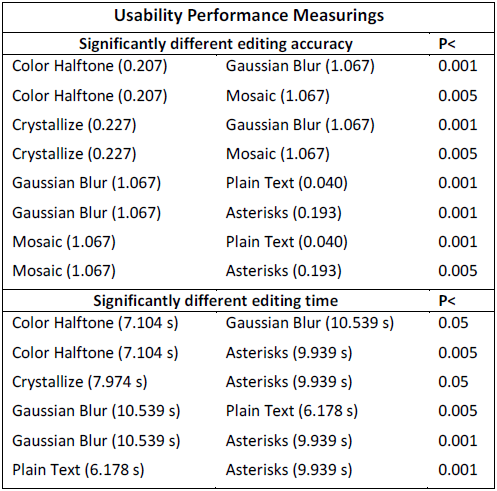
\includegraphics[width=\columnwidth]{figures/usabilityperformace_figure.png}
    \caption{Significant differences were found between the filter types above. The brackets show the mean values for editing accuracy on the right and editing time on the left}
    \label{fig:sig_table}
    \vspace{-5mm}
\end{figure}

The ANOVA also shows significant results for the editing task, where the test person has to edit the character x at specific position. We found a significant effect of filter types on the editing accuracy (F(5, 120) = 24.600, p $<$ 0.0005). Comparing the means based on the filter types, one can see that the Plain Text input performed the highest by accuracy, following by the Asterisks filter. Though, these outcomes were expected. Due to the task design the users could easily count the asterisk positions to insert the x, however, this does not really represent a use case which is why another editing task is conceivable for future investigations. Besides these results, the Crystallize and Color Halftone filters did perform satisfactorily accurate as well (see figure \ref{fig:sig_table}). The accuracy performance (editing accuracy) of the filters Gaussian Blur and Mosaic come off as lowest (see figure \ref{fig:sig_table}). That denotes that the users insert the x one position falsely next to the expected position on average. Overall, Gaussian Blur and Mosaic performed poorer than the other filters. 

Between the filter types significant differences in the editing time was found (F(5,120) = 6.447, p $<$ 0.005). Similar performing results as above was found. The users need the most time for the Gaussian Blur filter to edit the password, following by the Asterisks. The test persons score the fastest editing results for the Color Halftone and Crystallize filters (see figure \ref{fig:sig_table}). According to these outcomes, one could interpret that the classical authentication method is unsatisfying for editing task, like spelling corrections. Whereas the novel filter-based password technique is applicable for spelling corrections due to the readability for known words. According to the editing results, Color Halftone as well as Crystallize filters seem to be most promising. Future deeper investigations in editing task are required to have more precise results. 

Summing up, the filters Color Halftone and Crystallize achieve the best usability results. Gaussian Blur and Mosaic performed the worst in usability and therefore not applicable for the Password Blur concept. In the following section the results from the security task are discussed. 

\subsubsection{Results and Discussion - Security Task}
The evaluation of Task 2 showed that there is a significant effect of filter type on the Levenshtein distance between the participant's guess and the actual password (F(5, 120)=186.9,  p $<$ 0.001). As visualised in the graph below (see figure \ref{fig:levensthein}), the traditional Plain Text and Asterisks input methods show distinctly higher values in detectability under shoulder surfing attacks than the novel filter-based input methods.

The probability that a password can be obtained by third-parties is highest for Plain Text input (M=96,5\%, SD=4,37\%) followed by Asterisks input (M=86,8\%, SD=5,54\%) while the filter-based methods were much more secure from attacks with the following detectability values in descending order: Mosaic (M=55,8\%, SD=16,63\%), Gaussian Blur (M=38,9\%, SD=8,11\%), Color Halftone (M=31\%, SD=7,3\%) and Crystallize (M=23\%, SD=9,65\%).

These low values in readability for unknown entries based on filter-based input methods show that this novel authentication method is more secure and less vulnerable against shoulder surfing than classic input methods. Taking the example of choosing password phrases as a password type, which is recommended in recent publications \cite{shay2014can}, the guessability and chance that the password is obtained in case of a shoulder surfing attack with an asterisk-based (M=84,9\%, SD=8,66\%) input method is between 32\% (highest filter-based value: Mosaic, M=52,5\%, SD=17,67\%) and 68\% (lowest filter-based value: Crystallize, M=16,25\%, SD=1,06\%) higher than with a filter-based alternative. 

\begin{figure}[h]
    \centering
    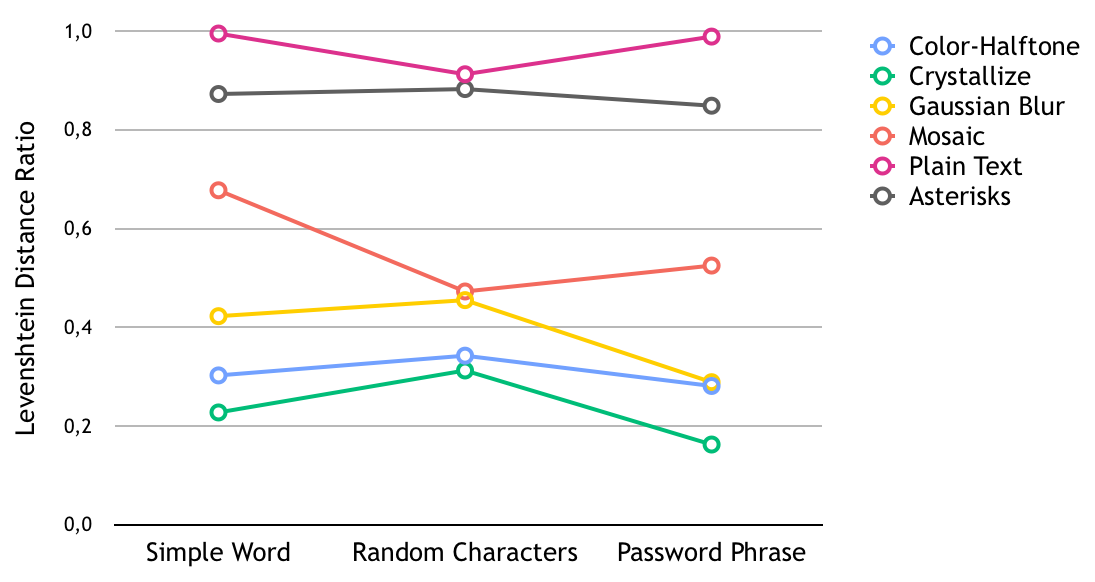
\includegraphics[width=\columnwidth]{figures/figure3.png}
    \caption{Average Levenshtein distance ratio depending on the word length for each password and filter type. Plain Text and Asterisks input methods show distinctly higher values in detectability under shoulder surfing attacks than the novel filter-based input methods
}
    \label{fig:levensthein}
    \vspace{-5mm}
\end{figure}

\subsubsection{Qualitative Interview}
In the concluding survey of our qualitative and quantitative study we were not only able to gather demographic information about our participants, but also insights about their subjective feelings while partaking in our study. On average our participants were 24 years old and like we already assumed more than two thirds are using password inputs on their mobile devices multiple times a week or more.

As security is nowadays an important topic, 84\% found it the easiest to read along the state of the art asterisks-based password input after they participated in the security part of our study. This shows, there is still potential for improvement for authentication on mobile devices. Moreover 60\% would use the password input based on degraded text on a daily basis. Reasons for this which was named are, inter alia, because it would be easier to correct typing errors and it would be harder for another person to read along.

When asked about the tradeoff between security and usability (which filter was the hardest to read along from a shoulder surfer perspective and at the same time was the easiest to correct) the participants liked the Crystallize filter of all filter types the most with a total of 36\% of all votes. 

\begin{figure}[h]
    \centering
    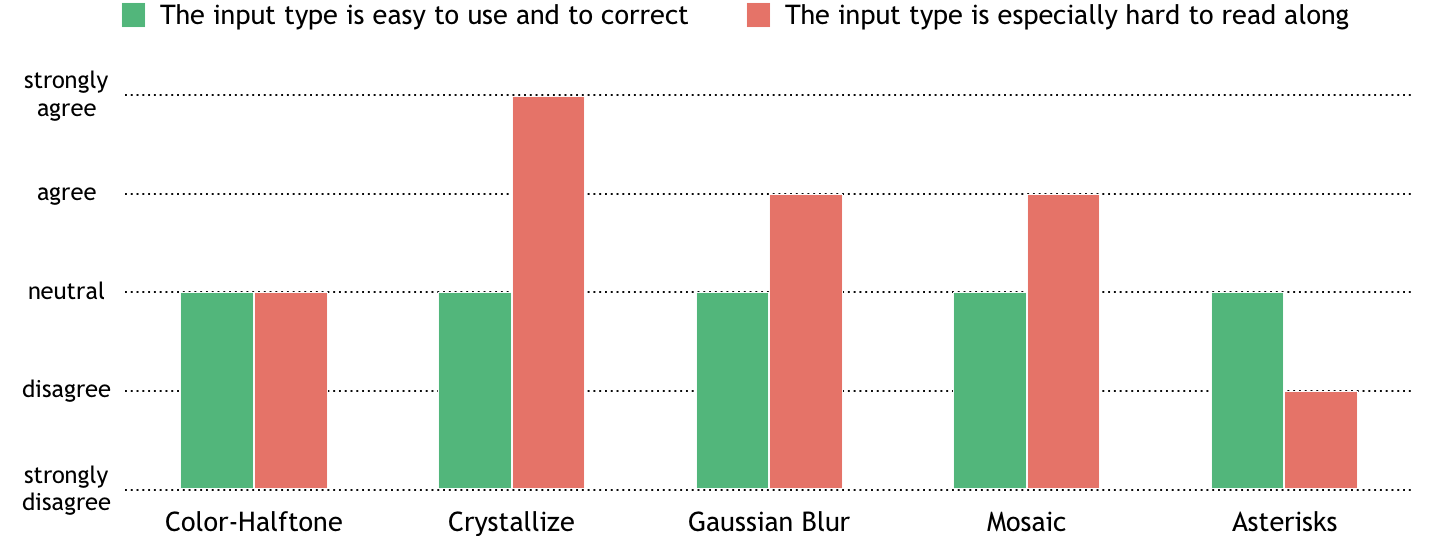
\includegraphics[width=\columnwidth]{figures/figure4.png}
    \caption{Median of the Likert scale: Perceived usability (green) and security (red) of different password input methods. While adding a character at a given position in the usability part of the study did feel the same for all filters, the participants found Crystallize, Gaussian Blur and Mosaic especially safe against shoulder surfing attacks in the security part}
    \label{fig:concluding_survey}
    \vspace{-3mm}
\end{figure}

To receive the participants subjective feeling which filter was good usability wise (easy to use and accurate in inserting an additional character at a given position) and which filter was secure against shoulder surfing we used a Likert scale from 1 (strongly agree) to 5 (strongly disagree), see figure \ref{fig:concluding_survey}.
The perceived usability among the different password filters and the asterisks-based input are the same and neutral. But in the perceived security there is a big difference. The participants strongly agree, that the Crystallize filter is especially hard to read along. They also agree, that the Gaussian Blur and Mosaic filters are secure against shoulder surfing. The feeling for Color Halftone is neutral and the interviewees think the asterisks-based password input is the weakest regarding the security.

Our data show, that the perceived feeling about the security of the different password input types is quite accurate as our password filters performed overall better in the second part of our qualitative and quantitative study.

\section{Conclusion}
To summarize, it can be stated that the filter-based authentication approach is less vulnerable against shoulder-surfing attacks but still performing at a constant high usability level and therefore a promising alternative to traditional input methods.

Comparing security and usability results we can see that the filters Color Halftone and Crystallize are most promising and therefore applicable for the Password Blur concept, that ensures a more usable as well as more secure approach for user authentication than the asterisk-based method. Password obscurations by Asterisks are the most observable based on the security study outcomes. This results due to the implementation of Android and iOS, that reveals the characters for a few milliseconds before hiding. Moreover, asterisks-based password inputs are not highly usable when it comes to spelling correction. Spelling mistakes are not able to be specifically detected, wherefore the user has to delete the whole input, which is time-consuming. With our filter-based method, users are faster detecting specific position of known words. Regarding this observation, Password Blur could provide the opportunity for a quick misspelling detection and correction, whereas the classical password input has its limitation. However, further investigation for this part is required to ensure high qualitative results. In summary, the conducted user study shows that filter types significantly influences editing accuracy and time (usability) as well as observation risks (security). On the basis of the study results, we would recommend the Crystallize filter to apply on the Password Blur method. 

\section{Future Work}
The results of both quantitative and qualitative data suggest great potential for this novel authentication method to enhance usability and security on mobile devices. A long-term field-study could be conducted among a larger number of people to get even sharper insights on the differences between the filters' gradations and the overall performance. Another interesting topic of research would be to evaluate this concept within the context of messaging \cite{eiband2016my}, where similar issues with regard to shoulder surfing are existing.


% Balancing columns in a ref list is a bit of a pain because you
% either use a hack like flushend or balance, or manually insert
% a column break.  http://www.tex.ac.uk/cgi-bin/texfaq2html?label=balance
% multicols doesn't work because we're already in two-column mode,
% and flushend isn't awesome, so I choose balance.  See this
% for more info: http://cs.brown.edu/system/software/latex/doc/balance.pdf
%
% Note that in a perfect world balance wants to be in the first
% column of the last page.
%
% If balance doesn't work for you, you can remove that and
% hard-code a column break into the bbl file right before you
% submit:
%
% http://stackoverflow.com/questions/2149854/how-to-manually-equalize-columns-
% in-an-ieee-paper-if-using-bibtex
%
% Or, just remove \balance and give up on balancing the last page.
%
\balance

\bibliographystyle{acm-sigchi}

\bibliography{sample}

%\begin{thebibliography}{1}

%\bibitem{stolz}
%K. Stolz, EyeVote: Experimenting with Voting on Public Displays via Gaze, Bachelorarbeit, Ludwig-Maximilians-Universität München, 2016

%\bibitem{perdis}
%M. Khamis, A. Bulling, K. Stolz, F. Alt, EyeVote: Exploring the Feasibility of Gaze-based Text Selection using Pursuits, Media Informatics Group, University of Munich, Germany,
%Perceptual User Interfaces Group, Max Planck Institute for Informatics, Saarbrücken, Germany, 2016

%\bibitem{fish}
%M. Khamis, F. Alt, A. Bulling. A Field Study on Spontaneous Gaze-based Interaction with a Public Display using Pursuits. UbiComp/ISWC Adjunct, 2015

%\bibitem{howto}
%F. Alt, S. Schneegaß, A. Schmidt, J. Müller, N. Memarovic, How to evaluate Public Displays, University of Stuttgart, Telekom Innovation Laboratories, TU Berlin, University of Lugano, 2016

%\bibitem{Muller:2012:LGF:2212776.2212488}
%J. Müller, R. Walter, G. Bailly, M. Nischt, Florian Alt, Looking Glass: A Field Study on Noticing Interactivity of a Shop Window, Quality and Usability Lab, Telekom Innovation Laboratories, TU Berlin, University of Stuttgart

%\bibitem{vidal}
%M. Vidal, A. Bulling, H. Gellersen, Pursuits: Spontaneous Interaction with Displays based on Smooth Pursuit Eye Movement and Moving Targets, UbiComp’13, Zürich, Schweiz, 2013

%\end{thebibliography}

\end{document}
